Copulas describe cross-market dependence, but they do not capture the temporal clustering of extreme events. In electricity markets, this temporal dimension is essential: once a market enters a stressed state, extreme prices often do not occur in isolation, but rather in bursts. For this reason, we model extreme events using Hawkes processes.

A Hawkes process is a self-exciting point process whose intensity depends on past events. In the multivariate setting, each component may also be excited by events occurring in the other component, which makes the framework particularly suitable for studying cross-market propagation. The process is stationary when the spectral radius of the branching matrix is strictly less than one.

\subsection{From hourly prices to event times}

Rather than modeling prices themselves as a point process, we transform the hourly time series into timestamped events. This is more natural in the Hawkes framework and better aligned with the objective of studying clustering in rare episodes.

We consider several event definitions, including negative prices, very high prices above the empirical 99\% quantile, large hourly jumps, and extreme spreads. In the final analysis, we focus on two economically meaningful cases: negative prices and very high prices. The negative-price case captures episodes of excess supply or severe market imbalance, while the high-price case captures upward stress episodes.

Table~\ref{tab:hawkes_event_counts} summarizes the frequency of the different event types.

\begin{table}[H]
\centering
\caption{Number and share of extreme events in France and Germany.}
\label{tab:hawkes_event_counts}
\begin{tabular}{lcccc}
\toprule
Event type & FR count & DE count & FR share & DE share \\
\midrule
Negative price      & 434 & 459 & 0.0741 & 0.0784 \\
High price 95\%     & 293 & 293 & 0.0500 & 0.0500 \\
Jump 95\%           & 293 & 293 & 0.0500 & 0.0500 \\
Spread extreme 95\% & 293 & 293 & 0.0500 & 0.0500 \\
High price 99\%     & 59  & 59  & 0.0101 & 0.0101 \\
\bottomrule
\end{tabular}
\end{table}

These frequencies justify the event-based approach. Negative prices are rare enough to be interpreted as stress events, but still numerous enough to support estimation. The same is true, more restrictively, for the upper 1\% price events.

\subsection{Univariate Hawkes analysis: negative prices}

We begin with univariate Hawkes processes estimated separately on the French and German negative-price events. We use an exponential kernel
\[
\phi(t) = \alpha e^{-\beta t}\mathbf{1}_{t>0},
\]
so that the branching ratio is given by \(\alpha/\beta\).

The observation window spans 6549 hours, with 434 negative-price events in France and 459 in Germany. Table~\ref{tab:hawkes_uni_negative} reports the corresponding estimates.

\begin{table}[H]
\centering
\caption{Univariate Hawkes estimates for negative-price events.}
\label{tab:hawkes_uni_negative}
\begin{tabular}{lccccccc}
\toprule
Country & \(\mu\) & \(\alpha\) & \(\beta\) & Branching ratio & \(\bar{\lambda}\) & Endogenous share & Log-likelihood \\
\midrule
France   & 0.0139 & 0.4935 & 0.6240 & 0.7909 & 0.0663 & 0.7909 & -1073.1962 \\
Germany  & 0.0148 & 0.5065 & 0.6415 & 0.7895 & 0.0701 & 0.7895 & -1119.8032 \\
\bottomrule
\end{tabular}
\end{table}

The baseline intensities are small in both countries, whereas the branching ratios are close to 0.79. This is a strong indication of self-excitation: once a negative-price event occurs, the probability of observing another similar event shortly afterward increases substantially. In both markets, roughly four-fifths of the total event activity is attributed to endogenous dynamics rather than to exogenous shocks.

This result confirms that negative prices are temporally clustered. They do not arrive as isolated points in time, but rather in bursts, which is exactly the kind of structure that a Hawkes process is designed to detect.

Figure~\ref{fig:hawkes_negative_timeline} presents the event raster plot over the full sample, while Figure~\ref{fig:hawkes_negative_intensity} shows the fitted univariate intensities.

\begin{figure}[H]
    \centering
    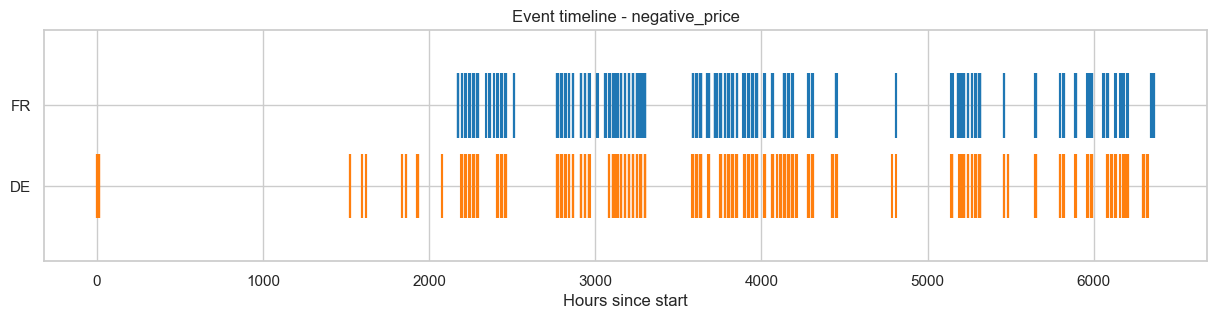
\includegraphics[width=0.8\textwidth]{figures/hawkes_negative_timeline.png}
    \caption{Timeline of negative-price events in France and Germany over the full sample.}
    \label{fig:hawkes_negative_timeline}
\end{figure}

\begin{figure}[H]
    \centering
    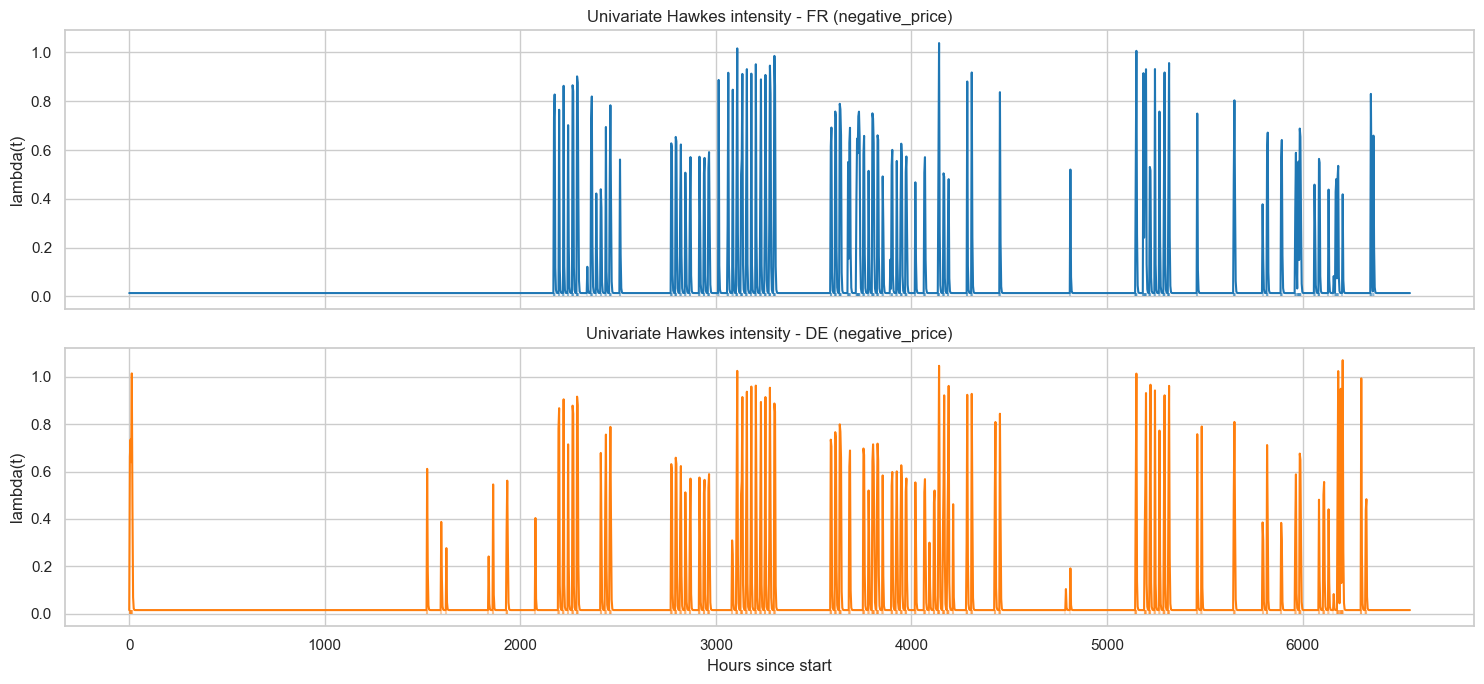
\includegraphics[width=\textwidth]{figures/hawkes_negative_intensity.png}
    \caption{Estimated univariate Hawkes intensities for negative-price events in France and Germany.}
    \label{fig:hawkes_negative_intensity}
\end{figure}

\subsection{Bivariate Hawkes analysis: negative prices}

We then estimate a bivariate Hawkes process in order to distinguish self-excitation from cross-excitation between the French and German markets. The fitted model yields the following branching matrix:
\[
G =
\begin{pmatrix}
0.6886 & 0.1321 \\
0.0308 & 0.7672
\end{pmatrix},
\]
with spectral radius
\[
\rho(G) = 0.8028 < 1.
\]

The stationarity condition is therefore satisfied. The model is stable, and the estimated long-run average intensities are \(\bar\lambda_{FR} \approx 0.0663\) and \(\bar\lambda_{DE} \approx 0.0701\).

Several features are noteworthy. First, both diagonal terms are large, which confirms strong self-excitation in each market. Second, cross-excitation is clearly asymmetric: the effect from Germany to France is larger than the reverse effect. More precisely, an extreme negative-price event in Germany appears to increase the short-term probability of a corresponding event in France more strongly than the opposite channel.

This asymmetry is economically plausible. It suggests that, for negative prices, the German market plays a stronger propagating role within the French-German pair. At the same time, the diagonal terms remain dominant, which means that local persistence is stronger than cross-border contagion.

Table~\ref{tab:hawkes_bi_negative} summarizes the bivariate estimates.

\begin{table}[H]
\centering
\caption{Bivariate Hawkes estimates for negative-price events.}
\label{tab:hawkes_bi_negative}
\begin{tabular}{lccc}
\toprule
Country & \(\mu\) & \(\bar{\lambda}\) & Endogenous share \\
\midrule
France  & 0.0114 & 0.0663 & 0.8283 \\
Germany & 0.0143 & 0.0701 & 0.7963 \\
\bottomrule
\end{tabular}
\end{table}

\begin{table}[H]
\centering
\caption{Estimated excitation matrix for negative-price events.}
\label{tab:hawkes_negative_matrix}
\begin{tabular}{lcc}
\toprule
Target / Source & FR source & DE source \\
\midrule
FR target & 0.6886 & 0.1321 \\
DE target & 0.0308 & 0.7672 \\
\bottomrule
\end{tabular}
\end{table}

Figure~\ref{fig:hawkes_negative_matrix} visualizes this excitation matrix, and Figure~\ref{fig:hawkes_negative_zoom} provides a zoom on the most tense week of the year.

\begin{figure}[H]
    \centering
    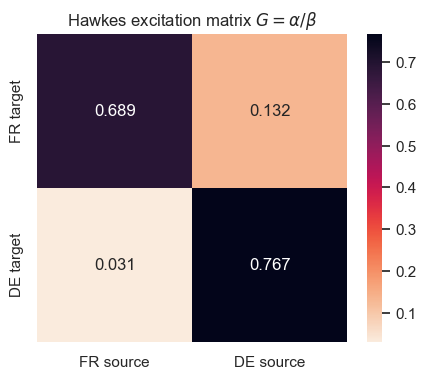
\includegraphics[width=0.45\textwidth]{figures/hawkes_negative_matrix.png}
    \caption{Estimated excitation matrix for the bivariate Hawkes model on negative-price events.}
    \label{fig:hawkes_negative_matrix}
\end{figure}

\begin{figure}[H]
    \centering
    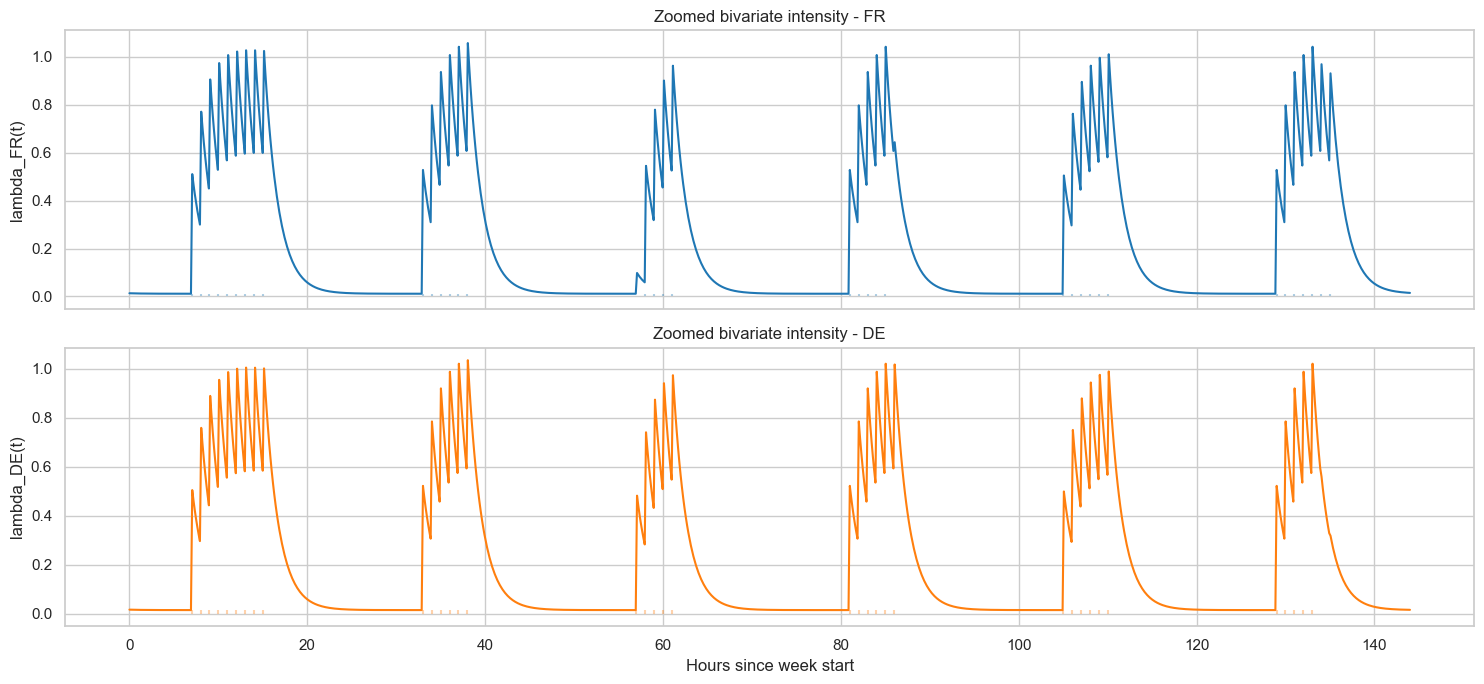
\includegraphics[width=0.8\textwidth]{figures/hawkes_negative_zoom.png}
    \caption{Zoom on a tense week for negative-price events and fitted bivariate intensities.}
    \label{fig:hawkes_negative_zoom}
\end{figure}

\subsection{Very high prices: upper 1\% events}

We perform the same analysis on very high prices, defined as observations above the empirical 99\% quantile. In this case, the observation window is again 6549 hours, but only 59 events are recorded in each country. These events are therefore much rarer than negative prices, which makes them especially relevant as indicators of severe upward market stress.

The univariate estimates are reported in Table~\ref{tab:hawkes_uni_high}. They again reveal self-excitation, with branching ratios of 0.8391 for France and 0.6663 for Germany.

\begin{table}[H]
\centering
\caption{Univariate Hawkes estimates for high-price 99\% events.}
\label{tab:hawkes_uni_high}
\begin{tabular}{lccccccc}
\toprule
Country & \(\mu\) & \(\alpha\) & \(\beta\) & Branching ratio & \(\bar{\lambda}\) & Endogenous share & Log-likelihood \\
\midrule
France   & 0.0014 & 0.1001 & 0.1193 & 0.8391 & 0.0090 & 0.8391 & -221.1900 \\
Germany  & 0.0031 & 0.1242 & 0.1864 & 0.6663 & 0.0093 & 0.6663 & -250.7652 \\
\bottomrule
\end{tabular}
\end{table}

The French series exhibits particularly strong self-excitation for upper-tail events. Once a very high price occurs in France, the fitted model indicates a high short-run probability of another high-price event shortly afterward. Germany also displays clustering, though less strongly.

The bivariate model leads to the branching matrix
\[
G =
\begin{pmatrix}
0.8271 & 0.0128 \\
0.1739 & 0.5234
\end{pmatrix},
\]
with spectral radius
\[
\rho(G) = 0.8343 < 1.
\]

Again, the stationarity condition is satisfied. The diagonal terms are large, especially for France, which confirms strong within-market clustering of upper-tail events. The cross-excitation terms are smaller than in the negative-price case and are also asymmetric, but now in the opposite direction: the effect from France to Germany is larger than the effect from Germany to France.

This difference between negative-price events and upper-tail events is particularly interesting. It suggests that the direction of cross-market propagation depends on the nature of the stress event. Negative-price episodes appear more strongly transmitted from Germany toward France, whereas very high price events appear more strongly transmitted from France toward Germany.

The corresponding summary tables are reported below.

\begin{table}[H]
\centering
\caption{Bivariate Hawkes estimates for high-price 99\% events.}
\label{tab:hawkes_bi_high}
\begin{tabular}{lccc}
\toprule
Country & \(\mu\) & \(\bar{\lambda}\) & Endogenous share \\
\midrule
France  & 0.0014 & 0.0090 & 0.8401 \\
Germany & 0.0028 & 0.0091 & 0.6957 \\
\bottomrule
\end{tabular}
\end{table}

\begin{table}[H]
\centering
\caption{Estimated excitation matrix for high-price 99\% events.}
\label{tab:hawkes_high_matrix}
\begin{tabular}{lcc}
\toprule
Target / Source & FR source & DE source \\
\midrule
FR target & 0.8271 & 0.0128 \\
DE target & 0.1739 & 0.5234 \\
\bottomrule
\end{tabular}
\end{table}

\subsection{Interpretation}

Taken together, the Hawkes analysis shows that extreme events are strongly clustered in time and exhibit measurable cross-excitation between the French and German markets. This cross-market propagation is asymmetric and depends on the event definition: negative-price episodes appear to spill over more strongly from Germany to France, whereas upper-tail events show the opposite pattern. In this sense, the Hawkes framework complements the copula analysis by adding a temporal dimension to joint extremes, showing that stress in the French-German day-ahead market is not only cross-sectional but also dynamically propagated over time.